\begin{frame}
\frametitle{\darkhighlightiii{Introduction: comparaison de systèmes linguistiques}}
%\pause
\begin{wideitemize}
\item Enjeux généraux en typologie linguistique
\begin{smallwideitemize}
  \item décrire des propriétés partagées par des systèmes
  \item {décrire les différences entre ces systèmes}
  \item développer le vocabulaire adéquat pour les caractériser
\end{smallwideitemize}
%\item Canonical typology in particular
%\pause
\item {Emploi de standards comparatifs}
%\pause
\begin{smallwideitemize}
\item Il existe plusieurs critères possibles parmi lesquels:
\begin{smallwideitemize}\footnotesize
  \item prototypicité, dérivable d'universaux linguistiques \cite{greenberg63}
  \item naturalité \cite{wurzel84,dressler00}
  \item {canonicité \cite{corbett03,corbett07b}}
\end{smallwideitemize}
\end{smallwideitemize}
% \pause
% \item \highlightii{\parsli}
% \begin{smallwideitemize}
% \item \highlightii{a formal approach to typology} w.r.t inflectional morphology.
% \item Development of measures for quantitave typological evaluation of
%   morphological systems.
% \end{smallwideitemize}
%\pause
\invisibletext{
\item[] {Canonicité --- approche autonome reposant sur un système
    d'ontologies}
\begin{smallwideitemize}
\invisibletext{
  \item[] la définition du canon repose sur des \invisibletext{propriétés définitoires}
  \item[] il est défini par un \invisibletext{espace multidimensionnel} des possibles
  \item[] il permet de comparer chaque système individuel en
    termes de \invisibletext{déviation plus ou moins marquée par rapport à un
      \invisibletext{étalon canonique}}
}
\end{smallwideitemize}
}
%\pause
%\item here: \highlighti{Canonical Inflection}
\end{wideitemize}
\end{frame}

\begin{frame}[t]{Qualifier la différence}
\begin{center}
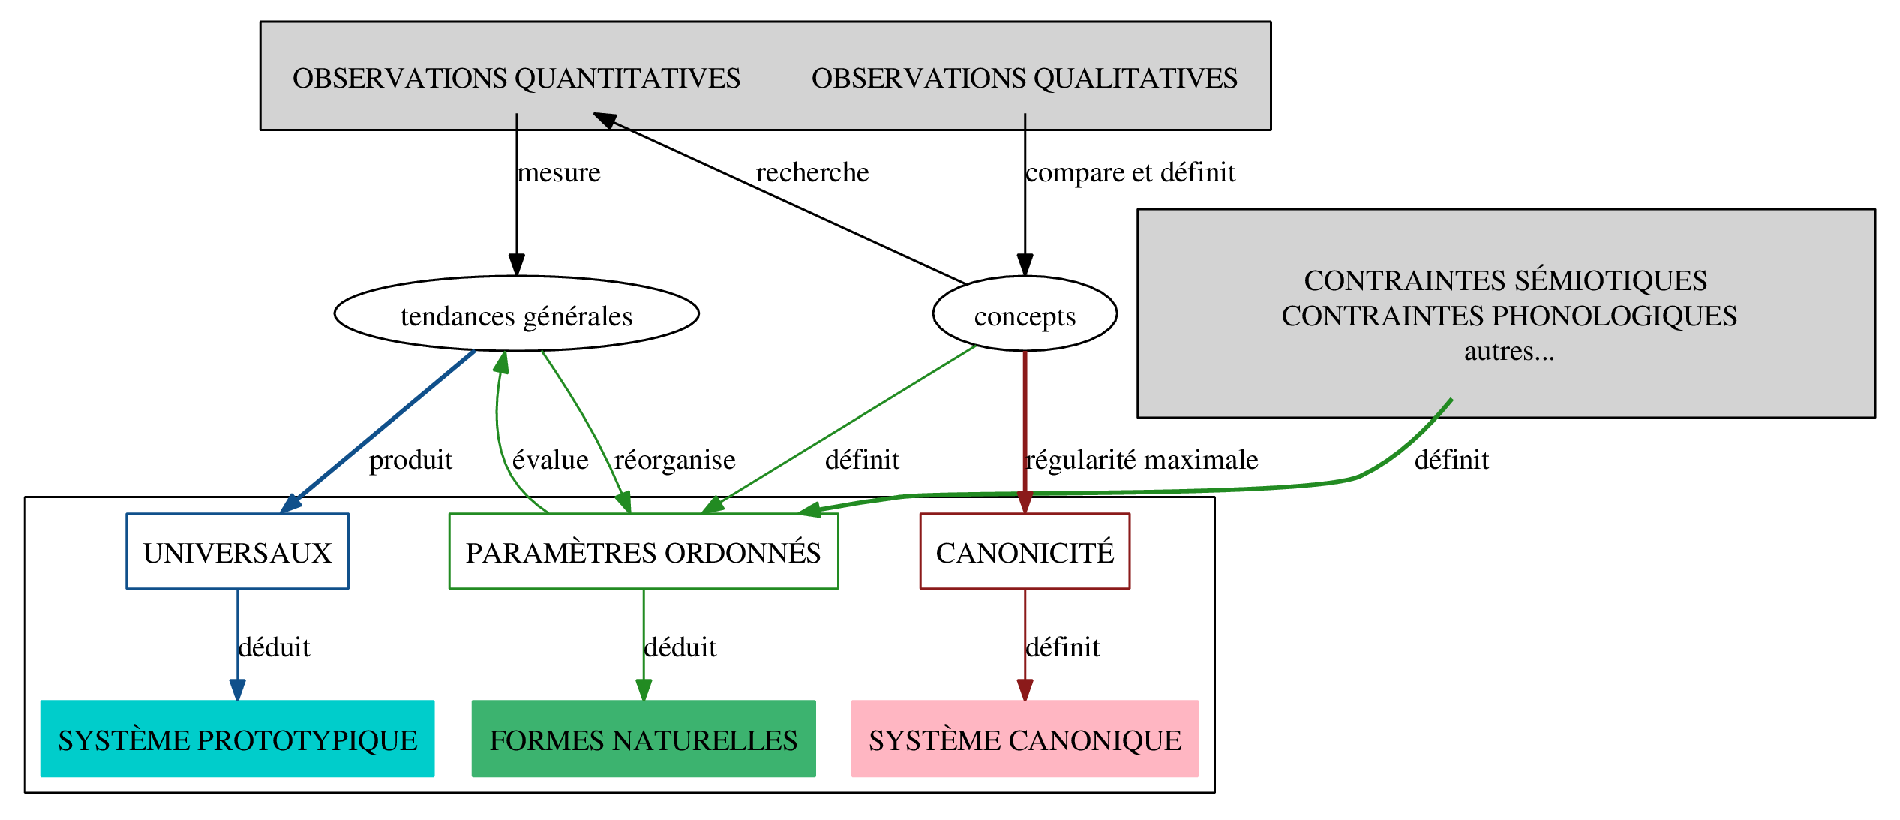
\includegraphics[width=120mm]{protonatcanon}
%\caption{Latin inflection zones}
\label{fig:canonicity}
\end{center}
\end{frame}

\begin{frame}
\frametitle{\darkhighlightiii{Comparaison de systèmes morphologiques}}
%\pause
\begin{wideitemize}
\item {Enjeux généraux en typologie linguistique}
\begin{smallwideitemize}
  \item {décrire des propriétés partagées par des systèmes}
  \item {décrire les différences entre ces systèmes}
  \item {développer le vocabulaire adéquat pour les caractériser}
\end{smallwideitemize}
%\item Canonical typology in particular
%\pause
\item {Emploi de standards comparatifs}
%\pause
\begin{smallwideitemize}
\item {Il existe plusieurs critères possibles parmi lesquels:}
\begin{smallwideitemize}
  \item {prototypes dérivables d'universaux linguistiques \cite{greenberg63}}
  \item {naturalité \cite{wurzel84,dressler00}}
  \item {canonicité \cite{corbett03,corbett07b}}
\end{smallwideitemize}
\end{smallwideitemize}
\pause
% \item \highlightii{\parsli}
% \begin{smallwideitemize}
% \item \highlightii{a formal approach to typology} w.r.t inflectional morphology.
% \item Development of measures for quantitave typological evaluation of
%   morphological systems.
% \end{smallwideitemize}
%\pause
\item Canonicité {\small --- approche autonome reposant sur un système
    d'ontologies}
\begin{smallwideitemize}
  \item la définition du canon repose sur des \lighthighlightiii{propriétés définitoires}
  \item il est défini par un \lighthighlightiii{espace multidimensionnel} des possibles
  \item il permet de comparer chaque système individuel en
    termes de \lighthighlightiii{déviation plus ou moins marquée par rapport à un
      \lighthighlightiii{étalon canonique}}
\end{smallwideitemize}
%\pause
%\item here: \highlighti{Canonical Inflection}
\end{wideitemize}
\end{frame}


\begin{frame}[t]{Représentation du canon selon Corbett {\em et al.} (2012) \nocite{corbett12imm}}
\begin{center}
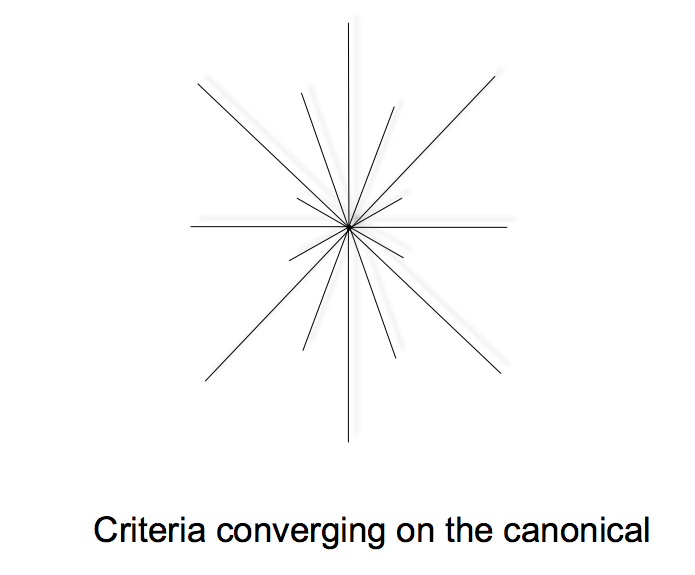
\includegraphics[width=80mm]{corbett-canon-star}
%\caption{Latin inflection zones}
\label{fig:canonicity}
\end{center}
\end{frame}